%% Standalone supplementary material: finite-strain neo-Hookean blobInTreacle, same-lineage cross-code check (FEniCSx against solids4foam PR #694).
%% Build (from this directory):  latexmk -pdf supplement_fenicsx_blobintreacle_neohookean.tex   (or pdflatex, bibtex, pdflatex, pdflatex)
%% It does not read article.aux (no cross-references to the main article), so it builds on its own.
%% Bibliography keys: Baratta2023 (DOLFINx) is in bibliography.bib (equal to main); PETSc, MUMPS:1, MUMPS:2, Cardiff2018 and Roache1998 are already there.
%% Data, scripts, provenance, bookkeeping and the audit response register: paper-data/fenicsx_blobintreacle_neohookean/ (README.md there).
\documentclass[sn-mathphys,Numbered]{sn-jnl}
\usepackage{graphicx}
\usepackage{amsmath,amssymb,amsfonts,bm}
\usepackage{xcolor}
\usepackage{soul}
\usepackage{manyfoot}
\usepackage{booktabs}
\usepackage{siunitx}
\usepackage{float}
\usepackage[utf8]{inputenc}
\usepackage[onehalfspacing]{setspace}
\usepackage{placeins}
\usepackage{geometry}
\geometry{a4paper,textwidth=15cm,textheight=24cm}
\setlength{\parskip}{0.2\baselineskip}
\raggedbottom

%% S-prefixed numbering
\renewcommand{\thesection}{S\arabic{section}}
\renewcommand{\thefigure}{S\arabic{figure}}
\renewcommand{\thetable}{S\arabic{table}}
\renewcommand{\theequation}{S\arabic{equation}}

\newcommand{\todo}[1]{\par\noindent\textcolor{red}{\rule{\linewidth}{0.8pt}}\par\nopagebreak
	\noindent{\small\color{red!70!black}\textbf{AUTHOR NOTE:} #1\par}\nopagebreak
	\noindent\textcolor{red}{\rule{\linewidth}{0.8pt}}\par}
\makeatletter
\renewcommand{\paragraph}[1]{\par\vspace{0.3\baselineskip}\noindent\textbf{#1}\ }
\makeatother
\newcommand{\FE}{FEniCSx}
\newcommand{\sfoam}{solids4foam}

\begin{document}
\clubpenalty=150 \widowpenalty=150

\title[Supplementary material: neo-Hookean blobInTreacle]{Supplementary material: finite-strain neo-Hookean blobInTreacle, a same-lineage cross-code check with a monolithic FEniCSx implementation}

\author*[1]{\fnm{Author} \sur{Placeholder}}\email{corresponding.author@example.org}
\author[1]{\fnm{Author} \sur{Placeholder 2}}

\affil[1]{\orgdiv{School of Mechanical and Materials Engineering}, \orgname{University College Dublin}, \orgaddress{\country{Ireland}}}

\maketitle

\todo{Placeholders: authors, CRediT, AI-use paragraph. Numbers come from the run records and CSV files in \texttt{paper-data/fenicsx\_blobintreacle\_neohookean/} (README files: provenance, archive, audit response register). \textbf{The solver repository and raw run output are not public}; only derived tables regenerate here. No manuscript section is changed.}

\section{Scope, claim level and disclosure}\label{sec:nh_scope}
The solids4foam tutorial \texttt{blobInTreacle} was redefined in solids4foam PR~\#694 to a finite-strain (total-Lagrangian, compressible neo-Hookean) solid. \textbf{This is a different mathematical problem from the historical linear-geometry blob} of the historical small-strain audit (\texttt{supplement\_fenicsx\_blobintreacle.tex}); the two are never mixed in one convergence sequence and no value of one serves as a reference for the other. This supplement gives a second implementation (monolithic finite elements, \FE{}) and a cross-code check against solids4foam at the pinned PR~\#694 head \texttt{6fa468d56503da711d09135599f85ab18f150513} (library source: merged \texttt{development} commit \texttt{206437983}). The solids4foam side was rebuilt and rerun unmodified and reproduces the PR-text numbers.

\textbf{Claim level.} A \emph{second implementation and cross-code check by the same group and the same AI lineage}, internal review only: not an independent verification, not external validation, and no claim of a defect in solids4foam. \textbf{Headline:} the five extrapolated limits ($u_x$, $u_y$, $F_x$, $F_y$, $\Delta p$) agree to $0.05$--$0.19\,\%$ with those of solids4foam, as differences between estimated limits, not absolute errors. Problem definition, mesh, observables, convergence routine, law and interface measure are shared with the solids4foam source, so a shared misreading would be invisible. \textbf{The preregistration was not blind} (Section~\ref{sec:nh_prereg}).

\section{Model, solver and meshes}\label{sec:nh_model}
\paragraph{Law.}
Total-Lagrangian compressible neo-Hookean solid with the three-dimensional isochoric split and $F_{zz}=1$ (plane strain):
\begin{equation}
W=\tfrac{\mu}{2}(\bar I_1-3)+\tfrac{K}{4}\left(J^2-1-2\ln J\right),\qquad
\bm\sigma=\tfrac{\mu}{J}\,\mathrm{dev}(\bar{\bm b})+\tfrac{K}{2}\,\tfrac{J^2-1}{J}\,\bm I,\qquad \bm P=\partial W/\partial\bm F,
\end{equation}
$\bar I_1=J^{-2/3}\operatorname{tr}(\bm F\bm F^{T})$ (with the $zz$ term), $\bar{\bm b}=J^{-2/3}\bm F\bm F^{T}$, $J=\det\bm F$, $\mu=50$~Pa, $\lambda=500$~Pa, $K=\lambda+2\mu/3=533.33$~Pa, $\rho_s=1$. The non-zero $\sigma_{zz}$ does not enter the in-plane balance, but the three-dimensional split is load-bearing. The tutorial's eight-digit $E,\nu$ give $K=533.33328$ ($10^{-7}$ relative; the \FE{} runs use the exact values).

\paragraph{Interface (M1).}
The solids4foam total-Lagrangian path applies the fluid traction per \emph{current} area (\texttt{useUndeformedArea} false by default, current normal in the traction gradient): the exact Nanson measure $\bm\sigma_f\,J\bm F^{-T}\bm N$ per reference area, equal and opposite forces on corresponding patches (M1 in the terms of the historical audit). The \FE{} model is M1 by construction.

\paragraph{Solver and levels.}
DOLFINx~\citep{Baratta2023} with PETSc SNES~\citep{PETSc} and MUMPS~\citep{MUMPS:1,MUMPS:2}; one monolithic system $(\bm u,p,\bm d)$ on one mesh, quadratic velocity and displacement, linear pressure, harmonic ALE mesh motion, BDF2 with a single backward-Euler first step; geometry, inflow and fluid as in the tutorial. Four quadrilateral levels $\times0.5,\,1,\,2,\,4$ of $150$, $600$, $2400$, $9600$ cells, identical in count and block topology to the solids4foam levels; steady \FE{} runs use $\Delta t=0.04$ to $t=6$ (agreeing with $\Delta t=0.02$, $0.01$ to $10^{-7}$ at $\times1$; see Section~\ref{sec:nh_time}), solids4foam $\Delta t=0.01$ ($0.005$ at $\times4$) to $t=3$. Orders and limits follow the main article (monotone, $0.5\le p\le3$, $F_s=1.25$~\citep{Roache1998}, $h=N^{-1/2}$); ``second order'' only for an accepted triple with $1.8\le p\le2.2$.

\section{Constitutive equivalence and solid-only gate}\label{sec:nh_law}
Over $20$ deformation gradients ($J$ from $0.09$ to $2.5$) the \FE{} law module has UFL-differentiated, analytic and numpy $\bm P$ in agreement to about $10^{-14}$, the UFL tangent equal to a finite-difference derivative to $3.6\times10^{-10}$, $\bm\sigma=\bm P\bm F^{T}/J$ to $6\times10^{-15}$, and objectivity to about $10^{-13}$. A C++ transcription of the solids4foam formulas agrees with it at identical $\bm F$ to $5.6\times10^{-15}$ ($\bm\sigma$) and $6.5\times10^{-15}$ ($\bm P$) with the solids4foam constants ($10^{-7}$ with the exact ones), and a separate re-implementation by an internal reviewer to $4\times10^{-16}$ (Cauchy) and $1.3\times10^{-9}$ (tangent) (\texttt{data/law\_checks.csv}).

\paragraph{Solid-only gate.}
A static half cylinder (no fluid, ALE or coupling), base fixed, follower pressure and $x$-traction per current area ($L1$: $10,\,5$~Pa; $L2$: $25,\,12.5$~Pa) was run in both codes with the real solids4foam law (\texttt{data/solid\_only\_differences.csv}). The apex $u_x$ of \FE{} relative to solids4foam is $-0.90$, $-0.52$, $-0.21$, $-0.10\,\%$ ($L1$) and $-1.97$, $-1.00$, $-0.45$, $-0.21\,\%$ ($L2$) on the four solid meshes, i.e.\ $0.1$--$0.2\,\%$ at $\times4$ and halving per refinement; the apex $u_y$ differs by $0.5$--$1.5\,\%$ without a clean trend. The \FE{} apex increments converge at observed orders $0.90$, $1.02$ ($L1$) and $0.69$, $0.74$ ($L2$) for $u_x$ and $0.7$--$0.9$ for $u_y$, while the solids4foam $u_x$ increments are non-monotone ($L1$) or irregular ($L2$: $1.0$, $2.9$). This \textbf{points toward a solid discretisation or boundary-regularity contribution} to the first-order apex displacement of the coupled runs (Section~\ref{sec:nh_steady}); the mechanism is not proven (a base-corner singularity is a candidate, not shown).


\section{Steady state: spatial levels and cross-code comparison}\label{sec:nh_steady}
\FE{} steady values at $t=6$ (drift over the last $0.5$ time units $\le5.3\times10^{-7}$; \texttt{data/fe\_steady\_levels.csv}): apex $u_x=0.13822$, $0.13929$, $0.13981$, $0.14006$~m at $\times0.5$ to $\times4$. The solids4foam rerun reproduces the PR text ($u_x$, $u_y$ at all levels, regression values, order $2.00$, extrapolated $0.14024$).

\begin{table}[!ht]
\centering
\caption{Matched-level differences (\%), (\FE{} steady $-$ solids4foam $t=3$)/solids4foam (\FE{} at $t=3$: $\le0.02$ pp change). \texttt{steady\_matched\_differences.csv}.}\label{tab:nh_matched}
\footnotesize
\begin{tabular}{@{}lrrrr@{}}
\toprule
 & $\times0.5$ & $\times1$ & $\times2$ & $\times4$ \\
\midrule
$u_x$ & $+10.71$ & $+2.74$ & $+0.53$ & $+0.083$ \\
$u_y$ & $+7.02$ & $+2.33$ & $+0.90$ & $+0.36$ \\
$F_x$ & $+11.43$ & $+2.94$ & $+0.56$ & $+0.037$ \\
$F_y$ & $+9.56$ & $+2.41$ & $+0.50$ & $+0.030$ \\
\bottomrule
\end{tabular}
\end{table}

\paragraph{Matched meshes.}
The $u_x$ difference shrinks by factors $3.9$, $5.2$, $6.4$ per refinement (Table~\ref{tab:nh_matched}; at $t=1$: $+7.85$, $+2.03$, $+0.40$, $+0.05\,\%$). The coarsest level differs by $7$--$11\,\%$, mostly coarse-mesh error of the cell-centred scheme (its $\times0.5$ $u_x$ is $11\,\%$ below its own limit, \FE{} $1.5\,\%$). Different discretisations (monolithic finite elements against cell-centred finite volumes with partitioned coupling) agree here: cross-code consistency, not proof of correctness of either.

\paragraph{Orders and estimated limits.}
Table~\ref{tab:nh_limits} gives the finest-triple order (coarse triple in brackets), limit and GCI of each code and the difference of the two estimated limits; all ten sequences are accepted. The orders differ: $u_x$ converges at $p=1.04$ in \FE{} ($1.05$ coarse) and at $2.00$ in solids4foam on the finest triple only ($1.62$ coarse); $u_y$ is near first order in both. In \FE{} second order holds only for $F_y$ ($2.03$; $1.93$) and, on the coarse triple, $F_x$ and $\Delta p$; the finest-triple $F_x$, $\Delta p$ orders ($2.66$, $2.47$) exceed $2.2$, so their GCIs of $0.005\,\%$ and $0.003\,\%$ are optimistic. The cause of the first-order apex displacement is not established (Section~\ref{sec:nh_law}).

\begin{table}[!ht]
\centering
\caption{Orders, limits and GCI (finest triple $\times1,2,4$; coarse triple in brackets; s4f: solids4foam); diff.: (\FE{} $-$ s4f)/s4f of the signed limits; in GCI: diff.\ over the root-sum-square of the two GCI; last column: diff.\ with fixed $p=1$ and $p=2$. \texttt{data/steady\_convergence.csv}, \texttt{limit\_sensitivity\_to\_order.csv}.}\label{tab:nh_limits}
\footnotesize
\setlength{\tabcolsep}{3pt}
\begin{tabular}{@{}lrrrrrrrrr@{}}
\toprule
 & \multicolumn{3}{c}{\FE{}} & \multicolumn{3}{c}{solids4foam} & diff. & in GCI & $p=1\ldots2$ \\
\cmidrule(r){2-4}\cmidrule(lr){5-7}
 & $p$ & limit & GCI (\%) & $p$ & limit & GCI (\%) & (\%) & & (\%) \\
\midrule
$u_x$ & $1.04\ (1.05)$ & $0.140302$ & $0.21$ & $2.00\ (1.62)$ & $0.140238$ & $0.26$ & $+0.046$ & $0.14$ & $-0.36\ldots-0.07$ \\
$u_y$ & $0.90\ (1.14)$ & $-0.014015$ & $0.84$ & $1.14\ (1.40)$ & $-0.014001$ & $1.16$ & $+0.10$ & $0.07$ & $-0.17\ldots+0.18$ \\
$F_x$ & $2.66\ (2.18)$ & $16.2408$ & $0.005$ & $2.17\ (1.71)$ & $16.2591$ & $0.19$ & $-0.11$ & $0.58$ & $-0.48\ldots-0.14$ \\
$F_y$ & $2.03\ (1.93)$ & $-25.6861$ & $0.005$ & $2.01\ (1.77)$ & $-25.7178$ & $0.20$ & $-0.12$ & $0.62$ & $-0.43\ldots-0.12$ \\
$\Delta p$ & $2.47\ (2.04)$ & $35.9868$ & $0.003$ & $1.76\ (1.76)$ & $36.0537$ & $0.32$ & $-0.19$ & $0.57$ & $-0.54\ldots-0.13$ \\
\bottomrule
\end{tabular}
\end{table}

\paragraph{What the limits do and do not show.}
With the preregistered rule (order from the data) the five limits differ by $0.05$--$0.19\,\%$ ($0.07$--$0.62$ of the combined GCI), and the \FE{} $u_x$ limit is $0.045\,\%$ from that of the PR-text sequence ($0.140239$). The result depends on the assumed order: for any fixed $p$ from $1$ to $2$ the difference is at most about $0.5\,\%$ ($u_y$ changes sign), and the matched $\times4$ values of the displacements and forces differ by $0.03$--$0.36\,\%$ ($\Delta p$ is compared at the limits only). The robust statement is agreement at the $\sim0.5\,\%$ level; the $\sim0.05\,\%$ reading holds only for the data-driven order. These are \emph{differences between estimated numerical limits, not absolute errors}: no analytical reference exists, the combined GCI is an estimate, not a bound, and the polygonal half circle common to both codes is unquantified. $\Delta p$ is the inlet minus outlet pressure (\FE{}: boundary mean of the inlet trace; solids4foam: inlet face value, equal to the adjacent-cell value for its zero-gradient inlet condition) and is compared at the extrapolated limits.

\begin{figure}[!tb]
\centering
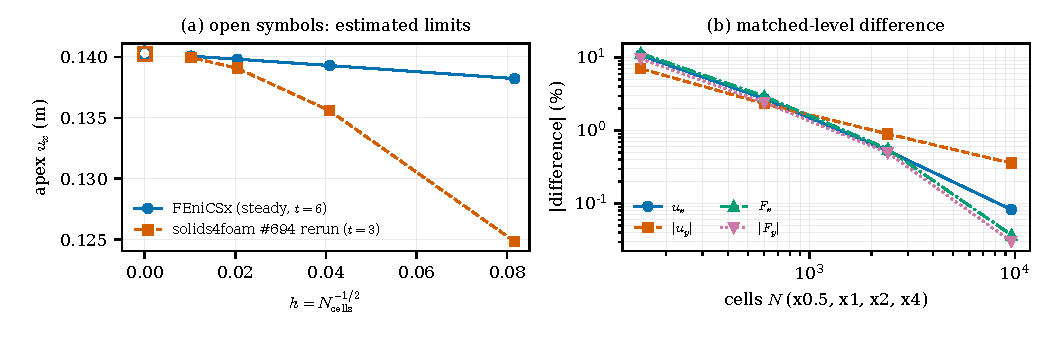
\includegraphics[width=0.78\textwidth]{paper-data/fenicsx_blobintreacle_neohookean/figures/nh_steady.pdf}
\caption{(a) Apex $u_x$ against $h=N_\mathrm{cells}^{-1/2}$ with the estimated limits (open symbols at $h=0$). (b) Magnitude of the differences of Table~\ref{tab:nh_matched}. \texttt{figures/nh\_steady.pdf}.}\label{fig:nh_steady}
\end{figure}

\section{Temporal study at \texorpdfstring{$t=1$}{t=1} and the failed order prediction}\label{sec:nh_time}
Six \FE{} and four solids4foam time steps on the $\times1$ mesh (Table~\ref{tab:nh_time}). The solids4foam orders of the successive $u_x$ and interface changes ($2.13$, $2.21$; $2.12$, $2.00$) reproduce the PR text; the \FE{} orders are $2.02$, $3.09$, $1.21$, $0.63$ and $2.02$, $2.70$, $1.30$, $0.68$. \textbf{The preregistered criterion V5 (first two orders in $[1.6,3.0]$) failed for $u_x$} ($3.09$) and stays failed; the interface orders pass; only the first pair agrees with solids4foam. The $u_x$ changes stagnate at $5.96\times10^{-6}$ and $3.85\times10^{-6}$~m ($9.8\times10^{-5}$ and $6.3\times10^{-5}$ relative) for $\Delta t\le0.0156$.

\begin{table}[!ht]
\centering
\caption{Time study at $t=1$ ($\times1$); $|\Delta u_x|$: change between successive $\Delta t$ (m). \texttt{data/time\_study\_t1.csv}.}\label{tab:nh_time}
\footnotesize
\begin{tabular}{@{}lrrrrr@{}}
\toprule
$\Delta t$ (s) & \FE{} $u_x(1)$ (m) & $|\Delta u_x|$ & s4f $u_x(1)$ (m) & $|\Delta u_x|$ & \FE{}/s4f$-1$ (\%) \\
\midrule
$0.25$ & $0.0602441$ & & $0.0590302$ & & $+2.06$ \\
$0.125$ & $0.0607231$ & $4.79\times10^{-4}$ & $0.0595007$ & $4.71\times10^{-4}$ & $+2.05$ \\
$0.0625$ & $0.0608409$ & $1.18\times10^{-4}$ & $0.0596084$ & $1.08\times10^{-4}$ & $+2.07$ \\
$0.03125$ & $0.0608547$ & $1.38\times10^{-5}$ & $0.0596316$ & $2.32\times10^{-5}$ & $+2.05$ \\
$0.015625$ & $0.0608607$ & $5.96\times10^{-6}$ & & & \\
$0.0078125$ & $0.0608645$ & $3.85\times10^{-6}$ & & & \\
\bottomrule
\end{tabular}
\end{table}

\paragraph{Excluded causes; open.}
A tighter SNES tolerance (Addendum~1) changes all five observables by at most $6.4\times10^{-12}$, so the stagnation is not a solver-tolerance floor; a $16$-substep first step (Addendum~2) gives the same orders ($1.80$, $3.11$, $1.16$, $0.71$), so the Euler start-up is not the cause. The cause is open. Against the finest run the $F_x$ error falls cleanly at second order, whereas the errors of $u_y$, $F_y$ and $\Delta p$ against the finest run change sign ($u_y$ between $0.125$/$0.0625$ and $0.03125$/$0.015625$; $F_y$ and $\Delta p$ twice, between $0.125$/$0.0625$ and $0.0625$/$0.03125$) and show a floor of $2$--$3\times10^{-4}$ (relative). \textbf{No second-order claim is made for all observables.} The \FE{}-to-solids4foam offset of $2.05$--$2.07\,\%$ is the same at every equal $\Delta t$ (Table~\ref{tab:nh_time}) and agrees with the $2.03\,\%$ spatial offset of the $\times1$ mesh to $0.04$ percentage points, so it is not a time-discretisation difference. SNES step-norm acceptances (reason 3; list in the README) occurred in $106$ steps of the $\Delta t=0.01$ steady run and in a few steps of four other runs, never at steady state; they qualify the steady $\Delta t$ independence ($\le1.0\times10^{-7}$) and the small-$\Delta t$ behaviour.


\section{Force closure and ALE quality}\label{sec:nh_force}
In \FE{} the fluid weak force on the solid equals the solid residual at the interface rows to $\le3\times10^{-10}$~N/m at every step of every run, the global solid momentum closure is $\le4.21\times10^{-10}$~N/m and the steady interface power $4.1\times10^{-7}$ at $\times1$. This is an algebraic identity of the weak form, not a check of the physics. The fluid-side integral and the weak force without the two corner dofs differ by $3.75$, $2.10$, $1.16$, $0.645\,\%$ in $F_x$ ($\times0.5$ to $\times4$), the corner-node share. The solids4foam interface balance of about $10^{-6}$ comes from the solids4foam authors' own runs and is \textbf{not reconstructed} here.

The minimum of $J$ over the run lies in the fluid ALE mesh: solid $0.75$, $0.64$, $0.51$, $0.35$ and fluid $0.68$, $0.60$, $0.46$, $0.19$ ($\times0.5$ to $\times4$); the minimum scaled Jacobian (fluid cells) is $0.68$, $0.65$, $0.61$, $0.32$ (sampled every ten steps; \texttt{data/ale\_quality.csv}). At $\times4$ the fluid $J=0.19$ is below the $0.2$ warning level used for the solid and had settled by $t\approx4$; its location was not logged. All sampled values are positive (every element valid), which does not establish mesh-independent accuracy.

\section{Preregistered predictions and chronology}\label{sec:nh_prereg}
The preregistration (SHA-256 \texttt{7106171b8a86}$\ldots$) and two addenda are in \texttt{preregistration/}. \textbf{Failed predictions are kept} (Table~\ref{tab:nh_prereg}).

\begin{table}[!ht]
\centering
\caption{Preregistered predictions (\texttt{data/preregistered\_scorecard.csv}).}\label{tab:nh_prereg}
\footnotesize
\begin{tabular}{@{}p{0.08\linewidth}p{0.42\linewidth}p{0.44\linewidth}@{}}
\toprule
Id & Prediction & Outcome \\
\midrule
P1 & $u_x$ within $3\,\%$ of s4f at every matched level, shrinking & \textbf{failed at $\times0.5$} ($+10.7\,\%$; not blind); met at $\times1,2,4$ \\
P3 & $F_x$, $F_y$ within $3\,\%$ & \textbf{failed at $\times0.5$} ($+11.4$, $+9.6\,\%$; not blind); met at $\times1$ ($2.94\,\%$), $\times2,4$ \\
P4 & $u_x(1)$ within $3\,\%$ at $\Delta t\le0.0625$, larger at $0.25$ & (a) met; \textbf{(b) failed} ($2.06\,\%$ at $0.25$) \\
P2, P5 & $u_y$ within $8\,\%$; \FE{} $u_x$ limit within $3\,\%$ of $0.14024$ & met ($7.0\,\%$ at $\times0.5$; $+0.045\,\%$) \\
V4 & orders: $u_x$, $F_x$, $\Delta p$ about $1.5$--$2$; $u_y$, $F_y$ $0.7$--$1.5$ & \textbf{$u_x$ failed} ($1.04$); $F_x$, $\Delta p$, $F_y$ above the range; $u_y$ met \\
V5 & first two time orders in $[1.6,3.0]$ & \textbf{failed for $u_x$} ($2.02$, $3.09$); interface met \\
V1--V3, V6, V7; A1, A2 & validity, drift, $\Delta t$ independence, closure, mesh quality; stagnation removed? & met (V7: $\times4$ fluid ALE warning); stagnation not removed \\
\bottomrule
\end{tabular}
\end{table}

\paragraph{Chronology (non-blind).}
Times are self-asserted, as logged on one machine. The solids4foam $\times0.5$ rerun finished at 20:51:55 ($u_x(1)=0.056168$) and an \FE{} $\times0.5$ smoke test ($u_x(1)=0.06058$) existed: about $+7.9\,\%$ at $\times0.5$ ($+2.0\,\%$ at $\times1$); the preregistration was hashed and committed at 20:55:28 and production submitted at 20:55:40. Addendum~1 was committed at 21:09:22 (jobs 21:09:28); for Addendum~2 the hash file, commit and job submission share the second 21:11:58, so its ordering cannot be shown. The predictions are scored as written and nothing in the preregistration was altered. \textbf{All of P1--P5 were set with the Phase 0 smoke results and the PR-text values in hand} (the solids4foam $\times1$ rerun finished at 20:54:44; the \FE{} $\times1$ smoke test showed $+2.0\,\%$); $\times0.5$ is where this was known to put P1 and P3 at risk, and the passes at $\times1,2,4$ are not blind tests either.

\section{Cost, tests and what is claimed}\label{sec:nh_claim}
The campaign used $11.23$ CPU-hours in $81$ Slurm jobs (peak $36$ cores): \FE{} $3.46$, solids4foam $7.54$ (including a cancelled attempt of $0.87$), small jobs and tests $0.23$; not an efficiency comparison. Legacy regression tests passed in the files run (evidence and counts in the README); the whole tree was \emph{not} run.

\textbf{Claim.} A monolithic \FE{} implementation of the finite-strain neo-Hookean blobInTreacle reproduces the solids4foam steady displacement and force limits within their reported combined numerical uncertainty: the five limits differ by $0.05$--$0.19\,\%$ for the data-driven orders and by at most about $0.5\,\%$ for any fixed order from $1$ to $2$; matched-mesh differences of the displacements and forces are $2.3$--$2.9\,\%$ at $\times1$ and $\le0.4\,\%$ at $\times4$ ($\Delta p$ is compared at the limits only). \textbf{Classification: qualified pass} (qualified cross-code consistency of the steady observables; temporal second-order convergence is not verified).

\textbf{Limitations.} Same group and AI lineage, internal review only; non-blind preregistration; the $u_x$ order $1.04$ and the time convergence below $\Delta t\approx0.016$ are unexplained; limits depend on the assumed order at the $0.1$--$0.5\,\%$ level; the $\times4$ ALE warning has an unknown location; point and integral observables of one benchmark; solver and raw output not public. A stronger statement needs external work.

\section*{AI-use disclosure (placeholder for author review)}
{\small\hl{TBD by the authors:} AI coding and writing assistants (Anthropic Claude) were used to implement and run the FEniCSx code, post-process and audit results internally and draft this text; the authors are to confirm, edit and take responsibility for the content and agree the wording with the journal's policy. No authorship is assigned to an AI system.}

{\small\bibliography{bibliography}}

\end{document}
